\section{Introduction}\label{sec:intro}

\ednote{very rought adapation of the introduction of my thesis; needs re-writing}

Mathematical knowledge bases are \ednote{continue definition}. 
These systems can range from calculators, which are only capable of performing simple computations, via mathematical databases (storing a set of a mathematical objects) to powerful modeling tools and computer algebra systems (CAS), that feature a broad variety of features.
A few examples of common MKS include the databases like \cite{oeis} and \cite{lmfdb}, systems like \cite{gap} and \cite{sagemath}, or the Wolfram Mathematica \cite{mathematica11} Computer Algebra System. 


Most of Mathematical Knowledge Bases are very specific -- they focus on one or very few aspects of mathematics. 
For example, OEIS is a database of integer sequences and nothing else, 
LMFDB is a database of objects in number theory. 
GAP excels at discrete algebra, whereas SageMath focuses on Algebra and Geometry in general. 

Being heavily specific, they usually focus on a specific data model that is exposed to users. 
In particular, \ednote{enum proper}
\begin{enumerate}
  \item these systems are usually only accessible to those familiar with the specific data representation; and
  \item different mathematical knowledge bases are non-interoperable programatically. 
\end{enumerate}

\ednote{Re-label this figure}
\begin{wrapfigure}{r}{0.25\textwidth}
  \begin{center}
    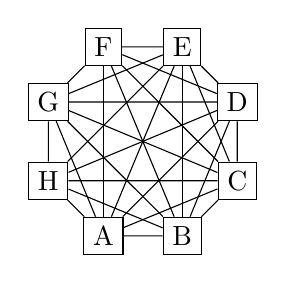
\begin{tikzpicture}
      \node[draw] (a) at (0,.3) {A};
      \node[draw] (b) at (1,.3) {B};
      \node[draw] (c) at (1.7,1) {C};
      \node[draw] (d) at (1.7,2) {D};
      \node[draw] (e) at (1,2.7) {E};
      \node[draw] (f) at (0,2.7) {F};
      \node[draw] (g) at (-.7,2) {G};
      \node[draw] (h) at (-.7,1) {H};
      \draw (a) -- (b) -- (c) -- (d) -- (e) -- (f) -- (g) -- (h) -- (a);
      \draw (a) -- (c) -- (h) -- (d) -- (g) -- (e);
      \draw (b) -- (h);
      \draw (b) -- (f);
      \draw (b) -- (d);
      \draw (b) -- (g);
      \draw (b) -- (e);
      \draw (h) -- (e);
      \draw (d) -- (f);
      \draw (g) -- (c);
      \draw (a) -- (d);
      \draw (a) -- (e);
      \draw (a) -- (f);
      \draw (a) -- (g);
      \draw (e) -- (c);
      \draw (c) -- (f);
    \end{tikzpicture}
  \end{center}

  \caption[Classical Approach to connecting systems]{
    Common Ad-Hoc Approach to Connecting Systems. 
  }
  \label{fig:classicalconnect}
\end{wrapfigure}


\ednote{Expand SOTA}
The State Of the Art for system interoperability is to export data from one system, convert it into a different format, and import it into a second system. 
This is usually achieved in an ad-hoc manner, that is programmers have to start from scratch each time they attempt to connect a new set of systems. 
If APIs exist, they only expose internal data structures of the individual components involved. 
Even though this enables interoperability, they only expose the internal database records, not the mathematical objects. e.g. elliptic curves over the rationals as number quadruples where each one of the numbers is represented as a string.

Attempting to connect $n$ systems usually means having to build in the order of $n^2$ such connections. 
This leads to a convoluted set of connections, seen in Figure~\ref{fig:classicalconnect}. 

\ednote{More expansion}
These interactions between MKB also lack in other aspects. 
In many scenarios, we want to compute with them, e.g. to find new relations between sequences in the OEIS (see~\cite{LuzKoh:fsarfo16}), or to find all elliptic curves in the LMFDB whose conductor is divisible by 5. 

We want to tackle this problem of making MKS interoperable, so we must make the content interoperable as well. 
Instead of exchanging low-level data structures, we propose to instead exchange semantic objects and only translate these to physical data structures inside the systems themselves. 
We call this the MiTM approach which we have introduced in \cite{DehKohKon:iop16}. 

The center of the MitM paradigm is the \textbf{Math-in-the-Middle ontology}, a flexiformal representation of mathematical knowledge, which is represented in the the \omdocmmt language, mechanized by the MMT system, and stored in the MathHub information system. 

\ednote{introduce mmt and data model (i.e. theories etc), along with MathHub}

To better represent MKS inside of MMT we introduce virtual theories. 
In a nutshell, virtual theories are just like concrete theories, but without the assumption of loading all declarations from a file on disk at system startup. 
Instead of loading all knowledge from an XML file, virtual theories load declarations in a lazy fashion when they are required. 
Here we do not even restrict ourselves to lazily reading an XML file, on the contrary, in most use cases we actually create the \omdocmmt\ representation on demand. 

 \ednote{Continue short outlook of schemas etc}

\subsection*{Structure}\label{sec:intr:structure}

